\chapter{インターネットプロトコル層(その1) インターネットプロトコルの概論}

この章では、インターネットプロトコルスイートにおける、インターネットプロトコル層について、概論的な説明をします。インターネットプロトコル層は、トランスポート層にどのようなサービスを提供するのでしょうか。そして、どのようにネットワークアクセス層を利用しているのでしょうか。

インターネットプロトコル層とは、その名の通り、複数のネットワークとネットワークの間で通信を行うためのプロトコルです。そして、TCP/IPのIPに相当するプロトコルでもあります。

何らかの機器をインターネット接続する際に、必ず、IPアドレスという言葉がでてきます。このIPとはInternet Protocolであり、略さずに言えば、Internet Protocol Addressとなります。では、インターネットプロトコルとはなにであるのか、そして、IPアドレスとは何であるのかを説明していくことにしましょう。

\section{異なるネットワークを結ぶ}

なぜインターネットプロトコル層が必要なのだろうか?ネットワークアクセス層の章を読み進めいていただいていたら、このような疑問を持たれるかもしれない。

そして、ネットワークアクセス層だけで世界中と通信すればいいのに、そうしない理由は何なのだろうか。

前章で説明したように、ネットワークアクセス層の物理的な規格とプロトコルには、いろいろなものがある。イーサネットは狭い範囲でホストの数が多い場合に向いているし、PPPは、距離にかかわらず、一対一接続を行う場合に向いている。

それなら、ネットワークアクセス層ごとに、プロトコル変換を行うものを置けばいいと思うかもしれない。だが、それなら、複数のネットワークを結ぶプロトコルを定めて、ネットワークアクセス層と、ネットワーク間のプロトコルを取り持つ機器にした方が汎用性が増すのではないだろうか。そして、ここでいうネットワーク間のプロトコルとは、インターネットプロトコルのことである。インターネットという言葉は、inter-net、つまり、ネットワークとネットワークの間なのだ。

\subsection{インターネットプロトコル層の昔話}

ここでも、インターネットプロトコル成立前夜の状況を振り返る昔話から始めよう。規格の由来というのは、全て昔話のなかに隠れているものなのだ。

後のインターネットに受け継がれる思想と技術は、1960年代後半から、アメリカの四つの大学を結ぶネットワークのARPANETからはじまった。

そんな中、ロバート・カーンは衛星パケット網と地上の無線パケット網の相互接続実験を行っていた。その過程で、カーンは、異なるネットワークの相互接続ができるということについての知見を得た。

今の用語で言えば、異なる構造のネットワークアクセス層同士の通信を行う、ということである。今となっては大げさでも何でもない。

一般的なインターネット接続は、LANとインターネット接続回線という、異なる構造のネットワークアクセス層どうしの通信を行っている。

TCP/IPの原初の形は1973年から1974年頃に、RFC675としてまとめられた。ALTO ALOHAがEthernetという名前になる前後の時代である。このころは、LANでも、ベンダーごとにまちまちな構造、規格、プロトコルを持つネットワークアクセス層掃討の規格が群雄割拠していた。

では、異なるネットワーク間で通信をするということは、どういうことであろうか。それは、それぞれの機器が直接に接続されているネットワークアクセス層の規格を問わず、エンドツーエンドでデータを届けるということである。だが、異なる構造のネットワークを越えて、通信するにはどうすればよいのだろうか。

それぞれのネットワークは、自分と、自分以外のネットワーク全てが、そのネットワークアクセス層では、宛先にフレームを届けることができることを期待する。もうひとつ、あるネットワークから来たデータグラムからデータを取りだして、宛先となるネットワーク宛のデータグラムに作り直して送る、中継の仕組みも用意しよう。この二つで、異なるネットワークの間で、とりあえずデータを相互に送りあうことができるのではないかと考えられる。

では、この異なるネットワークでデータを相互に送りあうこととはどういうことか、二つのネットワークを繋ぐところから初めて、順を追って説明していこう。

\subsection{二つのネットワークを結ぶ}

\begin{figure}[htbp]
	\includegraphics[width=12cm,clip]{draw/ip_basic2.eps}
	\caption{二つのネットワークを結ぶ}
	\label{fig:ip_basic2}
\end{figure}

まず、二つのネットワークを一つの中継役が結んでいる場合で考えてみよう。中継役はネットワークAとネットワークBとに接続されている。そして、それぞれのネットワークに対してネットワークアクセス層のプロトコルで通信することができる。

ネットワークAのホストからネットワークBのホストに宛てた通信は、とりあえず中継役に送る。中継役は、ネットワークB宛の通信が届いたら、ネットワークBのネットワークアクセス層のプロトコルで、宛先に通信を届ける。ネットワークBからネットワークAへの通信も同様である。

この中継役を置くメリットはなんであろうか。それは、それぞれのネットワークに属するホストが、自分の所属していない側のネットワークアクセス層の情報をもっていないくても、相互に通信が可能になるということである。つまり、自分以外のネットワークに関して、保持すべき情報がすくなくなる。つまりkじょれは、コンピュータのリソースを消費しないということでもある。

逆に、中継役は、中継に必要なアプリケーションのみ動作させる。そのため、リソースのほとんどを中継に使うことができる。役割を分担することで、全体の効率をあげることがでるというわけだ。

\subsection{三つ以上のネットワークを結ぶ}

つぎに、三つ以上のネットワークを結ぶ場合を考えてみよう。三つ以上のネットワークをそれぞれ中継役で結んでやる。ここでは、簡単にするために、図\ref{fig:ip_basic3}のようにネットワークが接続されているとしよう。

ネットワークAとネットワークB、ネットワークBとネットワークCの」間の通信は、先に説明したふたつのネットワークを接続した場合となる。では、ネットワークAとネットワークCの間の通信はどうなるのであろうか。

ネットワークAの中のホストは、宛先をネットワークCのホストにした通信を、ネットワークAとネットワークBの中継役に投げる。ネットワークAとネットワークBの中継役は、宛先がCであるのを確認すると、ネットワークBとネットワークCの中継役に通信を投げる。最終的に、ネットワークBとネットワークCの中継役が、ネットワークCに接続されたホストに中継する。

\begin{figure}[htbp]
	\includegraphics[width=12cm,clip]{draw/ip_basic3.eps}
	\caption{三つ以上のネットワークを結ぶ}
	\label{fig:ip_basic3}
\end{figure}

\subsection{もっとたくさんのネットワークが接続されている場合}

今度は、もっとたくさんのネットワークが接続されている場合について考えてみよう。つまり、実際のインターネットでどのように中継が行われるかを簡単に説明していく。

中継役は、自分が接続されているネットワークには自分で通信を中継する。そして、自分が接続されていないネットワークで、そのネットワークへの中継役と接続されていれば、その中継役に中継してもらう。

では、世界のどこかには存在するけれど、どこに存在するか知らない宛先と通信したいときはどうするか。中継役は、とりあえず自分が知らない宛先への中継を丸投げする、別の中継先というのを知っているとする。自分が知らない宛先への通信は、この「とりあえず」の中継先に丸投げする。

一見いい加減に思える方法であるが、インターネットの通信はこれで成り立っている。中継を繰り返すうちに、宛先へ向かう中継役を知っている中継役にいきつき、それを繰り返して、目的の宛先にたどり着くわけだ。いわばバケツリレーである。だが、廻されたバケツは自分の分かる範囲で適切と思われる宛先に渡す、という紳士協定に、すべての中継役は従っている。

\begin{figure}[htbp]
	\includegraphics[width=12cm,clip]{draw/ip_basic4.eps}
	\caption{もっとたくさんのネットワークを結ぶ}
	\label{fig:ip_basic4}
\end{figure}

\subsection{ルータ}
ここまで中継役という名前で説明してきたものが、現在ルータと呼ばれるものである。ルータは、届いた通信を、同じネットワークに接続されたホストを含む宛先に適切に中継するための機器である。

現在では一般家庭にも置かれるネットワーク機器であるブロードバンドルータも、その名の通り、家の中のネットワークとインターネットの間を中継する。

ルータと呼ばれるネットワーク間の中継専用の機器は、1990年代半ばにCisco Networksがはじめて発売した。それ以前は、PCやワークステーションにネットワークインタフェイスを複数取り付け、中継専用に使用することが多かった。

\subsection{デフォルトルートとルーティング}

ここまで、とりあえずの中継先として説明してきたものを、デフォルトルートと呼んでいる。デフォルトルートには、同じネットワークに宛先がない場合、宛先に接続されているルータを知らない場合に、とりあえず中継してもらうルータである。

ルータが一つだけ接続されているネットワークでは、そのルータが必ずデフォルトルートとなる。そのネットワークに接続されたホストは、そのルータをデフォルトルートとして設定することで、外部のネットワークとの通信が可能となる。

また、デフォルトルート以外のルータがあるときに、どのネットワークのホストと通信するときはどのルータに中継してもらう、という情報を、ルーティング情報やルーティングテーブルと呼ぶ。また、ルーティング情報に従って中継するルータを選択することを、ルーティングと呼ぶ。当然、デフォルトルートとの通信も、「知らない宛先」に対するルーティング情報に従ったルーティングであるといえる。


\subsection{遙かなるバケツリレー}

\begin{figure}[htbp]
	\includegraphics[width=12cm,clip]{draw/tier1.eps}
	\caption{Tier1プロバイダとプライベートピア}
	\label{fig:tier1}
\end{figure}


インターネットの通信とは、ここまで説明したバケツリレーを世界規模にしたものである。\footnote{CLANNADで、ことみのテディベアのエピソードを見ながら、IPのデータグラムと同じだと思ったのは筆者だけではないであろう。}デフォルトルートの役割を持つルータは、先に進むにつれて他のルータからもデフォルトルートにされる。そして、インターネットの全てのネットワークからのデータグラムがとりあえず届けられるルータは、全世界で25万ある経路について、次はどこに転送すればいいかを全て記憶している。

この全ての経路を、フルルートと呼ぶ。そして、フルルートを記録しているルータを管理するインターネットサービスプロバイダを、Tier1プロバイダと呼ぶ。

もっとも、Tier1以外のプロバイダの間で、プライベートピアと呼ばれるルーティングが設定されていることがある。これは、Tier1のプロバイダを介さずにその下位のISP同士でデータグラムを交換するための、専用線を使用した経路である。そのため、全てのデータグラムが必ず Tier1のルータを通過する、とは言い切れない。


\subsection{道はひとつではないが42通りあるとも限らない}

あるデータグラムが経由するルートは、実は毎回同じ経路を通って届く保証がない。あるデータグラムと、その次に届いたデータグラムは、それぞれ全く別の経路を通って届いた可能性がある。

これは、その時点でのネットワークの状況で経路を決める、ダイナミックルーティングを行うルータが経路の途中にあるためである。ダイナミックルーティングは経路に障害が発生していたり、負荷が高かったりするときに、転送する先のルータを変更する。そのため、データグラムの経路は送信毎に異なる可能性がある。また、経路が違えば送信した順番を崩して宛先に届くこともある。

インターネットプロトコル層には、データの送信順と受信順を保持し、一致させる機能は無い。もしそれが必要なら、トランスポート層以上でそれを担保するのがインターネットプロトコルスイートの考え方である。

インターネットプロトコル層が担当するのは、データグラムを宛先により近そうなルータに向けて転送することだけである。それ以上の、応答確認や到着したデータの順番の確認は、必要であれば、より上位のプロトコルが担当すべき仕事となる。


\subsection{何故世界はひとつのイーサネットではないのか}

ここまでの説明で、ルータでなくても、世界中イーサネットにしてブリッジで繋げばいいのではないか、そう思う読者諸兄がいるかもしれない。ここで、TCP/IPにおけるレイヤ以外の、ルータとブリッジの違いに触れておこう。

ルータもブリッジも、衝突ドメインか単一のネットワークかの違いはあるが、二つのネットワークに接続して中継を行うという点で、似た性質をもつ。だが、ルータにあってブリッジにない機能が、先に説明したルーティングである。ブリッジは直接接続された衝突ドメイン間での通信を可能とするだけである。そして、ブリッジで接続されたネットワークは、ここでいうひとつのネットワークとなり、物理的な大きさの限度が存在する。

だが、ルータは、適切なルーティングを行うことで、いくつものルータを介して接続された「遠隔」かつ「複数」のネットワークうに対して通信を行うことができる。ネットワークアクセス層よりも広い範囲で、ネットワークを越えた相互通信を行うためにインターネットプロトコル層が存在し、そして、そのための機器としてルータが存在するわけだ。

\subsection{インターネットプロトコルのアイディア}

ここまで説明したことが、大まかなインターネットプロトコルのアイディアである。話を戻せば、初期のTCPとIPは分離していなかった。ネットワークからネットワークにデータを転送する機能をインターネットプロトコル層として分離させたのは、TCPv3とIPv3という、TCP/IPのいわばバージョン3からである。

その後、IPのバージョンが4となる。このIPv4が、現在インターネットで使用されるアドレスと、それによる転送ルールなどの体系として、現在に至るまで30年以上使用されている。

現在は、IPv4と、その後継となるIPバージョン6、つまりIPv6とが併用されている。ここから、IPv4とIPv6について、変わらない部分、更新され、変更された部分のそれぞれを説明していくことにしよう。

\subsection{パケットとデータグラム}

インターネットプロトコル層のデータの単位を、パケットという。宛先情報であるヘッダと、データから構成されているのが、小包(パケット)とにていることから付けられた名前である。

パケットとは、元々は、電話のように、端から端まで物理的に回線を接続するコネクション型の通信と待避しての呼び方である。両端まで接続された回線をデータが流れるときは、「宛先」情報はいらない。なぜなら、送信する側の反対側が必ず宛先であるからだ。

だが、データに宛先情報を付加し、途中で宛先情報を参照して適切な宛先に転送する仕組みがあれば、たとえ送信側から受信側まで一本の経路が繋がっていなくても、そのデータはいつか宛先に辿り着くだろう。これが、、パケットの考え方である。ここまでの説明の言葉を使えば、宛先の書いてあるバケツということになる。

そのため、パケットを使う通信は、コネクション型通信に対比して、コネクションレス通信と呼ぶ。

また、インターネットプロトコル層の通信であることを強調したい場合は、IPデータグラムと呼ぶ。明らかにインターネットプロトコル層について語っている文脈では、単にデータグラムと呼ぶこともある。

\section{そもそもインターネットとは何か}

次に、インターネットという言葉に関する疑問を一つ晴らしておくことにしよう。
インターネットとインターネットプロトコル、言葉が似ているけれど何が違うのか、そんな疑問を持ちはしなかっただろうか。

インターネットとは、本来はこれから説明するIP(internet protocol)で接続されたネットワークのによって構成されるネットワーク事指す。

ここで気をつけるべきは、internet protocolを使用して相互接続される複数のネットワークなのでインターネットと呼ばれる、ということだ。インターネットで使用するプロトコルだから internet protocolなのではない。

\subsection{internnetとInternetの違い}

「インターネット」と読む語には、一般名詞としてのinternetと、固有名詞としてのInternetの二つが存在する。この二つの言葉には、それぞれどんな意味があるのであろうか。簡単にではあるが、辞書を引いてみることにしよう。

\begin{description}
\item[internet]単一の論理ネットワークを構築するために、共通のプロトコルで接続された複数の物理ネットワーク
\item[Internet]小文字で始まるinternetが相互接続された世界規模のネットワーク\footnote{定冠詞をつけてthe Netと表記する場合もある。}
\end{description}
アクセス
一般名詞のinternetは、この章で説明するインターネットプロトコルによって相互接続されたネットワークの集合遺体を指す。辞書的な意味に従えば、二つのネットワークアクセス層をインターネットプロトコルで相互接続すれば、それはもうinternetである。

固有名詞のInternetは、ARPAnetと呼ばれる、1969年に、アメリカで4つの大学を接続することから始まったネットワークの相互接続実験に端を発する。通常の教科書であればARPAnetのはじまりからTCP/IPの導入。発展的解消への歴史を説明すべきところであろう。だが、本書では、ARPAnetはTCP/IPに依って構築されたのでなく、1980年代初頭にARPAnetのプロトコルがTCP/IPに置き換えられた、という卵と鶏のどちらが先かの説明に留めておくことにする。\footnote{ARPAnetの歴史に興味があれば、参考文献に挙げた書籍を参照していただきたい。}




\section{インターネットプロトコル層}

ここまで説明したように、複数のネットワークアクセス層、つまり、物理ネットワークを相互接続するための層を、インターネットプロトコル層と呼んでいる。そして、インターネットプロトコルとは、インターネットプロトコル層で用いる通信規約である。では、ここから、インターネットプロトコルについて、もう少し立ち入って説明していくことにしよう。

インターネットプロトコルには、おおまかに、以下のような役目がある。本章では、この役目の一つ一つについて、説明を行っていく。

\begin{itemize}
\item ネットワークとホストを識別するための、インターネットプロトコルアドレスを定義する 
\item インターネットプロトコル層でのデータの単位であるデータグラムを定義する 
\item ネットワークアクセス層とトランスポート層を仲立ちする 
\item ルーティングする
\item データグラムにするには大きすぎるデータがきたとき、分割(フラグメント)する
\end{itemize}

\subsection{IPv4と」IPv6}
概論において簡単な説英を行ったが、現在、インターネットプロトコルにはバージョン4とバージョン6という二つのバージョンが存在する。

元々インターネットプロトコルスイートで用いられていたインターネットプロトコル層は、バージョン4である。だが、90年代に、バージョン4では、各ホストやネットワークを一意に区別するのに用いる番号、つまりIPアドレスが足りなくなることが予想された。そのため、取り得るIPアドレスの数を増やすことを第一の目的として策定されたのが、インターネットプロトコルのバージョン6である。IPv6では、アドレス数を増やす以外の拡張、変更も多く行われている。

本書第4版発行現在(2016年夏)はその過渡期であり、IPv4が主に使われている中、IPv6がアーリーアダプタから一般に広まりつつある段階である。

本書では、インターネットプロトコルのバージョン4をIPv4、バージョン6をIPv6と表記する。

\subsection{デュアルスタック}

IPv4とIPv6が併用されているということは、すなわち、現在、ふたつの「インターネットプロトコル」が併用されているということでもある。

つまり、インターネットプロトコル層の部分におさまるなにかが、二つ存在するということだ。では、この二つはどのような位置関係にあるのだろうか。

インターネットプロトコルスイートの菱餅重ねのなかにIPv4とIPv6をいれななおしてみると、図\ref{fig:dualstack}のように、二つのプロトコルが隣り合った位置に配置される。

トランスポート層は、このどちらの「インターネットプロトコル」も使うことができる。また、どちらのインターネットプロトコル層も、同様にトランスポート層にサービスをする。そして、どちらのインターネットプロトコル層も、ネットワークアクセス層からサービスを受ける。

つまり、実際のネットワークでは、IPv4とIPv6を同時に使うことができるということだ。このことを、インターネットプロトコル層のスタックが二つある、という意味で、デュアルスタックとよんでいる。

\subsection{デュアルスタックの優先順}

\begin{figure}[htbp]
	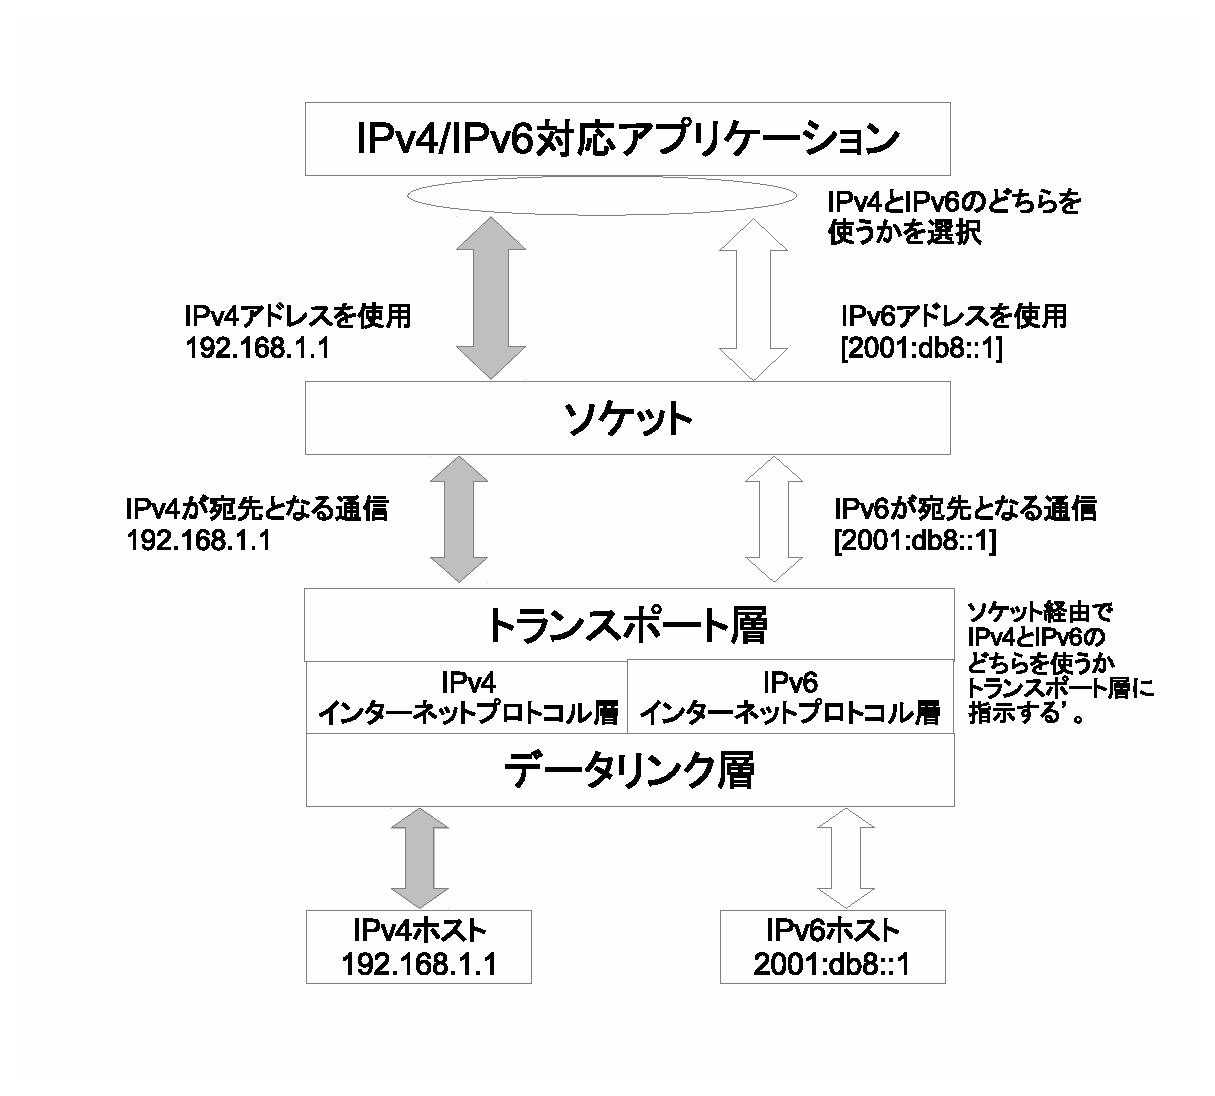
\includegraphics[width=12cm,clip]{draw/doublebind.eps}
	\caption{デュアルスタック}
	\label{fig:dualstack}
\end{figure}

デュアルスタックの環境かつ、IPv4とIPv6のどちらでも、同じホストに到達できる場合を考えてみよう。このとき、どちらのインターネットプロトコル層を使うのだろうか。

デュアルスタック環境では、まずIPv6によるアクセスが可能なら、IPv6でのアクセスを試みることになっている。IPv6での接続が規定の時間内に終了しない場合、あらためてIPv4でのアクセスを試みる。

実は、この選択を行うのはアプリケーション層である。実装上、アプリケーションがソケットを開くとき、アドレスファミリを選択することで、IPv4とIPv6のどチラを使うか、どちらから使うかを選択する。
IPv4のスタックはIPv4のスタックとしか通信できない。IPv6も、IPv6としか通信できない。インターネットプロトコル層には、どちらのスタックを使うべきかの判断をする自動判別のロジックは持っていない。


\section{インターネットプロトコルアドレス}

インターネットプロトコルという言葉で最初に思いつくものはなにであろうか。それはおそらく、インターネットプロトコルアドレス(Internet Protocol Address、以降IPアドレス)ではないだろうか。

IPアドレスとはその名の通り、インターネットプロトコルで接続されるネットワークにおいて、ホストとネットワークを識別するためにユニークにつけられる番号であり、これをアドレス\footnote{後で説明するように数字の列であるが、建物の号室表示までついた文字通りの住所と考えてよい。}と呼び表す。

\subsection{IPv4アドレスとIPv6アドレス}

先だって、インターネットプロトコル層として、二つのバージョンが併用されているという話をした。ということは、IPアドレスも、それぞれのバージョンに対応したものがあるということであろうか、そう考える読者諸兄もいるであろう。その予想は正しい。

IPアドレスは、最初は、IPv4の形式が実用化された。4組の数字をドットで区切った、192.168.1.1というような形式のアドレスである。
このIPv4でのIPアドレスは、32bitのビット列によって表される。数字表記は、人間が理解しやすいようにするために、先頭から8bitごとに区切って、それを十進数であらわしたものとなる。

つまり、IPv4アドレスは、0.0.0.0から255.255.255.255までのアドレスを取り得る。

では、IPv4アドレスはいくつ存在すのだろうか。IPv4アドレスは、32bit長なので、$2^{32}$個存在することができる。これを書き下すう4294967296個で、約43億個である。

一方のIPv6のアドレスは、128bitのビット列によって表される。これは、$2^{128}$個である。これを書き下すと、
340282366920938463463374607431768211456個
という膨大な数となる。

IPアドレスの総数と表記法は、IPv4とIPv6とで、一番わかりやすい相違と言えるだろう。まずそれを比較してみることにする。

このIPアドレスは、数字がドットで区切られてよっつ並んでいるだけに見える。だが、IPアドレスは単純な通し番号としてつけられているわけではない。まずはIPアドレスの構造について説明しよう。

IPv4アドレスは、32bitのビット列で表される。それを分かりやすくするために、8ビット毎に区切って10進数にして、ドット区切りで記述する。\footnote{IPv6では、128bitを16bitづつコロン:で区切り、その区切られたものを16進表記する。} おそらく、192.168.0.1というような記述をされているIPアドレスを目にしたこともあるであろう。アドレスの種類としては、特別な意味があるので割り当てないものなども含めて、0.0.0.0から255.255.255.255まで$2^{32}$通りの記述が可能である。

一方のIPv6は、128bitを16bitづつコロンで区切り、その区切られたものを16進表記する。4桁の16進数が8個並ぶものとなる。たとえば、2001:0db8:0000:0000:0000:0000:0000:0001というような表記となる。そのため、IPv6のアドレスには、省略記法が定められている。その省略記法に従えば、先のアドレスは2001:0db8::1と記述することができる。
この省略記法については、後ほど改めて説明する。



\subsection{IPv4アドレスは多いのか少ないのか}
IPv4のアドレスは、$2^{32}$個存在することができる。後述するように、特別な意味があって割り当てないアドレスも含めて、およそ43億個のアドレスである。果たして、このアドレスは多いのだろうか、それとも少ないのだろうか。

実は、2016年8月現在、APNICからアジア太平洋地区に新たに割り当てられるIPアドレスはない。割り当てを受けたインターネットプロバイダが配布するものがあるだけである。なのはでもまどかでもなく、IPアドレス完売、である。一方アメリカのIPアドレスを管理するARINにはIPv4割り当てに余裕がある。そのため、アメリカのインターネットサービスはIPv6への対応が遅いという別の問題もある。

43億個のアドレスは、世界中にインターネット接続可能な機器が存在する現在、とても足りるわけがない数である。
とはいえ、TCP/IPの実用化が始まった時代には、十分に多かったことも事実である。何より、アドレスなんかに4オクテット分も、貴重な通信時間を割いていたのだ。では、その当時、IPアドレスを持っていたホストが世界中でいかにに少なかったかの話をしよう。

Unixの/etc/hostsは\footnote{Windowsにも該当するhostsファイルが存在する}、DNS開発以前に、ARPAnetに接続されていた全ホストの情報をFTPで配布していた名残である。このファイルは、当時のARPAnetに新しいホストが追加される毎に、FTPで新しいものが配布されていた。IPv4実用化の頃は、4億個というのが永遠に使い切ることがないと思えた、途方もないアドレス数であったことが伺えるエピソードである。

一方のIPv6のアドレス数$2^{128}$個は、いまのところ十分に多い数である。よく使われる例えとして、地球上の砂粒全てにIPアドレスを割り当てられるという表現がされることもある。\footnote{ひとつのネットワークに割り当て可能なホスト数だけでも、およそ$1.84*10^{19}$個という膨大な数となる。}

\subsection*{}
\begin{itembox}[l]{いもうとコラム IPsec}
インターネットプロトコル層での通信に、認証と暗号化のオプションを付加するセキュリティ関連の規格に、IPsecがあります。IPv4では後付けの機能でしたが、IPv6では必須となりました。

IPsecは、インターネットプロトコル層のペイロードに認証ヘッダを付けたり、暗号化したりします。そのため、トランスポート層以上で何を使っているのかにかかわらず利用できます。

IPsecについての詳細は、それだけで専門書も多く出ているので、そちらを参照してください。


\end{itembox}